\paragraph{}
The SBFEM developed by Song and Wolf \citep{Wolf1996} provides a promising semi-analytical method to analyze problem in fracture mechanics and unbounded domain.
As a method developed based on the FEM and the BEM, the SBFEM is a fundamental-solution-less boundary element method which keeps the benefits of the both as well as provides some effective solutions to the limitations to the FEM and the BEM \citep{Wol1999}.
In contrast to the FEM, only the boundary is discretized using the conventional FEM interpolating function which leads to a decline in the number of unknowns.
It also allows solving the problem involving bimaterial interfaces and crack faces without the discretization of them.
Compared to the BEM, the fundamental solution is no longer required.
The infinite boundary can be achieved naturally as the radiation condition at infinity is satisfied in the SBFEM \citep{Wol2003}..

\paragraph{}
Fig.~\ref{lr_fig:sbfem_intro} illustrates a basic concept of the SBFEM.
A scaling center $O$ is selected at a point from which the whole boundary of the domain is visible (scaling requirement).
This condition is automatically satisfied for all convex polygons and many concave polygons.
The scaling requirement is equivalent to the notion of ``star convexity'' \citep{Bishop2014}.
For the domain that does not meet the scaling requirement, the requirement can always be satisfied by sub-structuring, i.e. dividing the structure into smaller subdomains, for example, scaled boundary polygon formulation \citep{NATARAJAN2014101}.
The problem domain can be covered by scaling the boundary in the radial direction respect to the scaling center with a ratio $\xi \in [0,1]$.
In the domain, only the boundary at $\xi=1$ is discretized with the conventional shape functions.

\begin{figure}[!ht]
    \centering
    \scalebox{0.5}{
        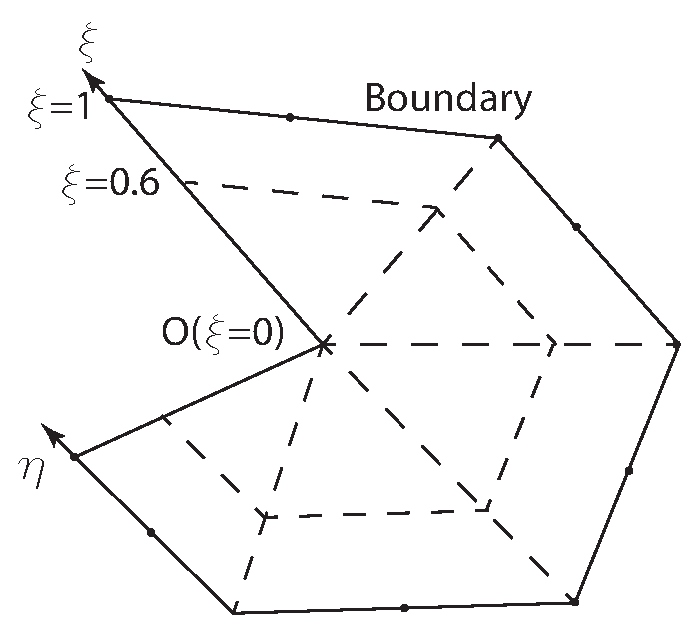
\includegraphics{literature/images/sbfem_intro.eps}
    }
    \caption[Two dimensional scaled boundary coordinates]{Two dimensional scaled boundary coordinates, where O is the scaling center and $\xi$ is the radial coordinate with $\xi=0$ at the scaling center and $\xi=1$ on the boundary.}
    \label{lr_fig:sbfem_intro}
\end{figure}
% \FloatBarrier
\paragraph{}
The method proved to be far more versatile and was applied to static problems in bounded domains and extended to take into account prescribed displacements \citep{DEEKS20041153} and concentrated loads \citep{Vu2014}.
A simple derivation of the necessary equations based on the virtual work principle is also presented \citep{Dee2002}.
This spurred the interest among researchers, as the similarity with the virtual work-based FEM derivation was highlighted.
The method is further developed by deriving a stress recovery technique that was later adopted in adaptive refinement techniques, such as h- and p-adaptive SBFEM \citep{NME:NME439, doi:10.1002/nme.440, Vu2008441, YANG20111417}.
The wave interaction with a cylindrical structure is investigated \citep{TAO2007232} and the method is also extended to structural dynamics \citep{Song2009} where the dynamic stiffness matrix was obtained as a continued fraction solution.
The main advantage of this approach is that the inertial effect at high frequencies can be modeled by high-order terms of the continued fraction without introducing an internal mesh.
A higher order spectral element was used in computation of the dispersion curves of the elastic wave using the SBFEM \citep{GRAVENKAMP201446} and a superior accuracy compared to the conventional approaches is shown.

\paragraph{}
The conventional FEM is known to be inefficient to deal with internal discontinuities such as material interfaces or singularities.
In an effort to overcome the limitations of the FEM, mesh-free methods and enrichment techniques such as the extended finite element method (XFEM) were introduced.
Treatment of evolving discontinuities in mesh-free methods \citep{doi:10.1002/nme.1151,Rabczuk2007} and enrichment techniques \citep{Babuška20031,doi:10.1002/nme.1966,CHAUDINH2012242,AREIAS2013113} is more straightforward because it does not require conforming mesh or frequent mesh adaptation as the discontinuities evolve.
On the other front, by exploiting the unique feature of the scaling center, the method allows the computation of stress intensity factors directly from their definitions \citep{Dee2005,SONG2002183}.
This has emerged to be an attractive alternate to the already established methods such as the XFEM and the meshless methods to model crack propagation.

\paragraph{}
Chidgzey et al. \citep{CHIDGZEY20081198,BIRD2010599} coupled the SBFEM with the BEM for computations in fracture mechanics.
This framework combines the semi-analytical solution accuracy of the SBFEM with the geometric flexibility provided by the BEM.
Natarajan and Song \citep{doi:10.1002/nme.4557} combined the extended FEM and the SBFEM, thus, circumventing the need to know a priori the enrichment functions, required by the former.
Recently, Ooi et al. \citep{doi:10.1002/nme.4284} and Natarajan et al.\citep{NATARAJAN2014101} employed scaled boundary formulation in polygonal elements to study crack propagation and compared the performance with other displacement based formulations, respectively.
Li et al.\citep{LI201352} applied SBFEM to analyze two-dimensional fracture problems in piezoelectric materials.
Ooi et al.\citep{doi:10.1002/nme.4284,OOI20101178,OOI20131} developed an efficient methodology for automatic crack propagation simulation using the SBFEM.

\paragraph{}
It can be seen that, since the inception of the method, the SBFEM has been applied to various problems in engineering and science.
It should be noted that most of the above studies employed Lagrange interpolants to approximate the unknown fields in the circumferential direction. He et al.
\citep{HE201228,HE2014152} employed moving least square (MLS) shape functions and Fourier series expansion to approximate the displacement fields in the circumferential direction.
It should be noted that the MLS and Fourier basis functions do not satisfy Kronecker δ property and that special care must be employed to enforce the boundary conditions.
It was shown that the SBFEM with MLS and Fourier shape functions yielded more accurate results than the MLS.
Very recently, Lin et al.\citep{Lin2014} employed non-uniform rational B-splines to approximate the unknown field in the circumferential direction.
However, their study was limited to 2D elastostatics.
